\usetikzlibrary{calc}


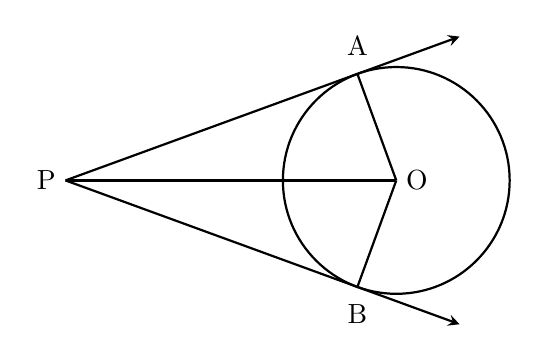
\begin{tikzpicture}[scale=1.2, >=stealth]
    % 1. Define Geometric Parameters
    \def\radius{1.2cm}
    \def\dist{3.5cm} % Distance from Center to P
    \coordinate (O) at (0,0);
    \coordinate (P) at (-\dist, 0);

    % 2. Calculate Tangent Points A and B mathematically
    % The angle of the radius OA relative to the line PO is acos(R/dist)
    % Since P is on the negative x-axis, we adjust angles for Quadrants 2 and 3
    \pgfmathsetmacro{\angle}{acos(\radius/\dist)} 
    
    \coordinate (A) at ({180-\angle}:\radius);
    \coordinate (B) at ({180+\angle}:\radius);

    % 3. Draw the Main Shapes
    % Circle
    \draw[thick] (O) circle (\radius);

    % Radii OA and OB
    \draw[thick] (O) -- (A);
    \draw[thick] (O) -- (B);

    % Center Line PO
    \draw[thick] (P) -- (O);

    % Tangent Lines (Extending past A and B)
    % We draw from P through A/B and extend by a factor of 1.3
    \draw[thick, ->] (P) -- ($(P)!1.35!(A)$);
    \draw[thick, ->] (P) -- ($(P)!1.35!(B)$);

    % 4. Add Labels
    \node[right] at (O) {O};
    \node[left] at (P) {P};
    \node[above=3pt] at (A) {A};
    \node[below=3pt] at (B) {B};

\end{tikzpicture}